\documentclass[10pt]{article}
\usepackage[a4paper,margin=18mm,top=16mm,bottom=16mm]{geometry}
\usepackage[scaled=0.92]{helvet}\renewcommand{\familydefault}{\sfdefault}
\usepackage[T1]{fontenc}\usepackage{amsmath,booktabs,array,xcolor,titlesec,enumitem,caption,float}
\usepackage{pgfplots}\usepgfplotslibrary{groupplots}\pgfplotsset{compat=1.15}
\titleformat{\section}{\normalsize\bfseries}{\thesection}{0.6em}{}\titlespacing*{\section}{0pt}{10pt}{3pt}
\setlength{\parindent}{0pt}\setlength{\parskip}{3pt}\captionsetup{font=small,labelfont=bf,skip=4pt}
\setlist{nosep,leftmargin=1.2em,itemsep=3pt}\pagestyle{empty}
\definecolor{ink}{HTML}{0B0B0B}\definecolor{muted}{HTML}{52514E}\definecolor{gridc}{HTML}{DDDCD6}\definecolor{bandc}{HTML}{EEEDE8}
\definecolor{otherc}{HTML}{A3A29B}\definecolor{cA}{HTML}{2A78D6}\definecolor{cB}{HTML}{EB6834}\definecolor{cC}{HTML}{1BAF7A}
\pgfplotsset{
  other/.style={otherc, line width=0.5pt, mark=*, mark size=1.1pt, mark options={fill=otherc, draw=white, line width=0.2pt}},
  hi/.style={line width=1.1pt, mark=*, mark size=1.9pt, mark options={draw=white, line width=0.4pt}},
  sA/.style={cA, mark options={fill=cA, draw=white, line width=0.4pt}},
  sB/.style={cB, mark options={fill=cB, draw=white, line width=0.4pt}},
  sC/.style={cC, mark options={fill=cC, draw=white, line width=0.4pt}}}
\begin{document}
{\large\bfseries What we compare against what, and why the vertex cap moves out of the RD figure}\\[1pt]
{\small All numbers are measured runs. 13 Nov 2026.}

\section{Two questions, answered separately}
\begin{itemize}
\item \textbf{Is the codec good?} Take the same meshes and change only the codec. Our files are 2.4 to 2.5 times smaller than TFAN's. This is the only comparison where nothing but the codec changes.
\item \textbf{Is the whole system good?} In the RD figure, TFAN needs 4.1 to 8.2 times more bytes than we do for the same PSNR. This number is larger than the codec gain because it also includes the gain from training the mesh at the target size. It is a system comparison, not a codec comparison, and the paper will say so.
\item \textbf{Where does the vertex cap go?} Out of the RD figure and into the ablation table. At the same file size we are 0.33\,dB above the cap (better in 34 of 36 comparisons). A gap of 0.33\,dB cannot be seen in a plot that spans tens of MB, which is why the orange curve did not look higher than the blue one. The cap row uses our codec and is trained at the target size, so it is our own system with one part swapped. It is an ablation, not an outside baseline.
\end{itemize}

\section{The vertex cap does not decide the file size}
Each line in Figure~\ref{fig:cap} is one scene. Every scene in a panel is plotted on the same cap axis.

\begin{figure}[H]\centering
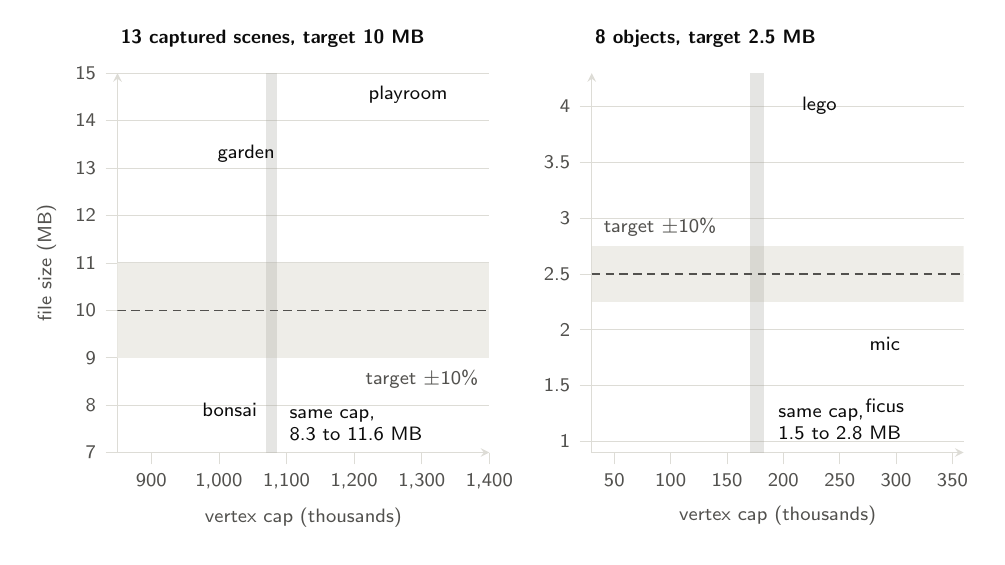
\begin{tikzpicture}
\begin{groupplot}[group style={group size=2 by 1, horizontal sep=13mm}, width=0.52\textwidth, height=64mm,
  axis lines=left, axis line style={gridc}, tick style={gridc}, tick align=outside, tick label style={font=\scriptsize, text=muted, /pgf/number format/assume math mode=true},
  title style={font=\scriptsize\bfseries, text=ink, at={(0,1)}, anchor=south west, inner sep=1pt, yshift=2pt},
  label style={font=\scriptsize, text=muted}, ymajorgrids, grid style={gridc, line width=0.3pt}, clip=true, clip marker paths=true,
  xlabel={vertex cap (thousands)}, scaled ticks=false, /pgf/number format/1000 sep={,}]
\nextgroupplot[title={13 captured scenes, target 10 MB}, xmin=850, xmax=1400, ymin=7, ymax=15, ylabel={file size (MB)}, xtick={900,1000,1100,1200,1300,1400}, ytick={7,8,...,15}]
\path[fill=bandc] (axis cs:850,9) rectangle (axis cs:1400,11);
\path[fill=otherc, fill opacity=0.28] (axis cs:1069,7) rectangle (axis cs:1086,15);
\draw[muted, line width=0.5pt, dash pattern=on 3pt off 2pt] (axis cs:850,10) -- (axis cs:1400,10);
%%CAPTURED%%
\node[font=\scriptsize, text=muted, anchor=north east] at (axis cs:1398,8.95) {target $\pm$10\%};
\node[font=\scriptsize, text=ink, anchor=east] at (axis cs:1097,13.30) {garden};
\node[font=\scriptsize, text=ink, anchor=north east] at (axis cs:1071,8.25) {bonsai};
\node[font=\scriptsize, text=ink, anchor=west] at (axis cs:1207,14.55) {playroom};
\node[font=\scriptsize, text=ink, anchor=south west, align=left] at (axis cs:1090,7.05) {same cap,\\8.3 to 11.6 MB};
\nextgroupplot[title={8 objects, target 2.5 MB}, xmin=30, xmax=360, ymin=0.9, ymax=4.3, xtick={50,100,150,200,250,300,350}, ytick={1,1.5,...,4}]
\path[fill=bandc] (axis cs:30,2.25) rectangle (axis cs:360,2.75);
\path[fill=otherc, fill opacity=0.28] (axis cs:170,0.9) rectangle (axis cs:183,4.3);
\draw[muted, line width=0.5pt, dash pattern=on 3pt off 2pt] (axis cs:30,2.5) -- (axis cs:360,2.5);
%%OBJECTS%%
\node[font=\scriptsize, text=muted, anchor=south west] at (axis cs:32,2.75) {target $\pm$10\%};
\node[font=\scriptsize, text=ink, anchor=south east] at (axis cs:256,3.84) {lego};
\node[font=\scriptsize, text=ink, anchor=north] at (axis cs:290,2.02) {mic};
\node[font=\scriptsize, text=ink, anchor=north] at (axis cs:290,1.47) {ficus};
\node[font=\scriptsize, text=ink, anchor=south west, align=left] at (axis cs:187,0.93) {same cap,\\1.5 to 2.8 MB};
\end{groupplot}
\end{tikzpicture}
\caption{File size against vertex cap, one line per scene, every cap run in the plotted range. Three scenes per panel are coloured, the others are grey. Dashed line and light band: target and $\pm$10\%. Dark vertical strip: the cap at which every scene of the panel was trained.}\label{fig:cap}
\end{figure}

What the figure shows:
\begin{itemize}
\item \textbf{Same cap, different scenes, different sizes.} With a cap of about 1.08 million vertices the 13 captured scenes give files from 8.3 to 11.6\,MB. With a cap of about 176 thousand the 8 objects give files from 1.5 to 2.8\,MB.
\item \textbf{Same scene, almost the same cap, different sizes.} Garden: a cap of 1,104,000 gives 13.3\,MB and a cap of 1,105,000 gives 10.3\,MB.
\item \textbf{A larger cap can give a smaller file.} Bonsai: 1,005,000 gives 9.6\,MB, 1,073,000 gives 8.3\,MB.
\item \textbf{Raising the cap can do nothing.} Mic stays at about 2.05\,MB from a cap of 134 thousand up to 247 thousand. Ficus stays at 1.5\,MB from 97 thousand up to 515 thousand.
\end{itemize}

\begin{table}[H]\centering\small
\begin{tabular}{@{}lrrl@{}}
\toprule
scene & cap & file (MB) & what happened \\
\midrule
garden & 1,104,000 & 13.30 & \\
garden & 1,105,000 & 10.30 & cap +0.1\%, file $-$23\% \\
garden & 1,106,000 & 10.15 & \\
\addlinespace
playroom & 1,080,000 & 10.37 & \\
playroom & 1,081,000 & 10.96 & cap +0.1\%, file +6\% \\
\addlinespace
bonsai & 1,005,000 & 9.57 & \\
bonsai & 1,073,000 & 8.32 & cap +7\%, file $-$13\% \\
\addlinespace
drjohnson & 902,000 & 11.69 & \\
drjohnson & 1,081,000 & 11.57 & cap +20\%, file $-$1\% \\
\addlinespace
lego & 130,000 & 2.50 & \\
lego & 142,000 & 2.40 & cap +9\%, file $-$4\% \\
lego & 154,000 & 2.79 & cap +8\%, file +17\% \\
lego & 183,000 & 2.79 & cap +19\%, file unchanged \\
\addlinespace
mic & 133,718 & 2.07 & \\
mic & 247,000 & 2.05 & cap +85\%, file $-$1\% \\
\bottomrule
\end{tabular}
\caption{Examples from the figure, each row compared with the row above it.}
\end{table}

Over all cap runs, counting pairs of runs on the same scene:
\begin{itemize}
\item caps less than 1\% apart: 11 pairs. In 4 of them the larger cap gave the smaller file. In 2 the file changed by more than 10\%.
\item caps less than 5\% apart: 29 pairs. In 12 the larger cap gave the smaller file. In 8 the file changed by more than 10\%.
\end{itemize}

\section{What this means for hitting a size}
21 scenes, one target each: 10\,MB for the 13 captured scenes, 2.5\,MB for the 8 objects. ``Ours'' measures the real file every 500 training steps and removes whatever is above the target; one training per scene.
\begin{table}[H]\centering\small
\begin{tabular}{@{}lcc@{}}
\toprule
 & Vertex cap & Ours \\
\midrule
Cap chosen from & other scenes, same dataset & not needed \\
Within $\pm$10\% after 1 training & 15 / 21 & 20 / 21 \\
Within $\pm$10\% after 3 trainings & 18 / 21 & -- \\
Within $\pm$2\% after 1 training & 3 / 21 & 16 / 21 \\
Never within $\pm$10\% & drjohnson, mic, ficus & ficus \\
PSNR at the same file size & reference & +0.33\,dB (34 of 36) \\
\bottomrule
\end{tabular}
\end{table}
\vspace{-4pt}
The cap baseline was given its best case: a cap taken from scenes of the same dataset and up to three trainings. We propose to stop here. Any further variant of the cap baseline would be a new method that we design ourselves, so its result could always be questioned.
\end{document}
